\chapter{Result and Evaluation}

In this chapter, the results of the optimized prediction hyperparameters and the robust range of the association hyperparameters are presented. In \Sec{1d}, the effects of all tracking hyperparameters are first examined with grid search. The effects of some hyperparameters are explained, and the most effective hyperparameters and their range for the optimization are also presented in this section. In \Sec{validation}, the Bayesian optimization method is verified to be able to reconstruct the hyperparameters in the system. In \Sec{Tests of Bayesian Optimization} and \ref{Test of Different Materials}, the selected hyperparameters are optimized with Bayesian optimization for all the datasets from real materials, and the difference of the optimized value of hyperparameters are discussed. In \Sec{Robust Range of Association Hyperparameters}, the general effects of each association hyperparameter are first examined with grid search. Then the SVMs showing the robust range of the hyperparameters are trained with the tracking results from the DEM dataset. The effect of the hyperparameters is also discussed at the last of the section.

\section{Optimization of the Hyperparameters of Motion Prediction}
\label{opt pred}
\subsection{General Effect of the Hyperparameters}

% \subsubsection{Grid Search}
\label{1d}
\subsubsection{Result of 1-D Grid Search}

% \textcolor{red}{added a introduction here two paragraphs.}
As mentioned in the last chapter, grid search on the datasets with two motion models was performed at the start of the optimization process. The aim of grid search is to give the initial knowledge of the effect of each hyperparameter. The most important hyperparameters and their ranges for optimization were obtained from this knowledge. For the CV model, the prediction hyperparameters include the measurement variance $S^{\boldsymbol{v}}$, the system noise variance $S^{\boldsymbol{w}}$ and the initial variance for position and velocity, as shown in Table \ref{list hp cv}. For the CVA model, the prediction hyperparameters include the variance for position, velocity and angle in the measurement, prediction and initialization steps, as shown in Table \ref{list HP cva}. In this section, the hyperparameters were checked separately, which means only the hyperparameter for checking would be changed in the search, and all the other hyperparameters remained as default values.

% \textcolor{red}{Is it necessary to give a table for the list of hyperparameters here? I think it's too long and adding a link/reference to the table in chapter 3 or 5 is enough?}


 

% However, in order to avoid the interference of the association errors, the distance appear at middle $d_{\mathrm{am}}$ was set at 15 in this section. The effect of changing this hyperparameter is shown in Figure \ref{meacov}. The association error rate is significantly reduced, especially when the measurement variance is lower than 10. The prediction error is also reduced since the false association increases the number of tracks, with which summation of the prediction error of all tracks also increases.

% \textcolor{red}{Changing the asso HP here doesn't really change the prediction error of each tracks. But because of the wrong association the number of tracks is increasing. Therefore, the total error increases and the $E_{\mathrm{p}}$ increases. $E_{\mathrm{p}}$ equals to the summation error of all the tracks in the test result dividing the track number in the reference result  $E_{\mathrm{p}}=\frac{\sum d_{i}^{\mathrm{Err}}}{n_{ref}}$. So I think it's not good to use something like "the mean error in each tracks increasing", because it's only the number of tracks increasing. In fact, if I divide the summation of error to the actual track number in the test result, the $E_{\mathrm{p}}$ decreases even if there is more tracks.}

\begin{figure}[htbp]
\centering
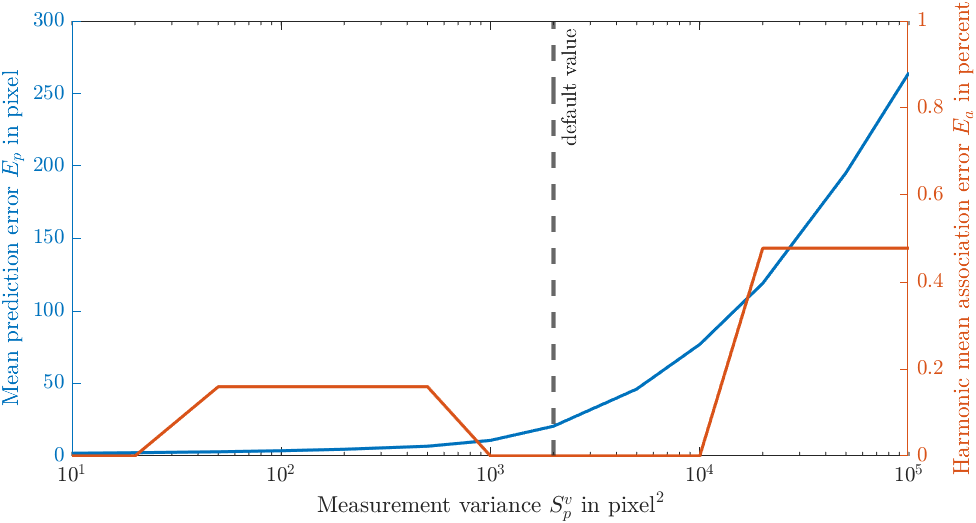
\includegraphics[width=0.9\textwidth]{figures/KF/meacov pfeffer cv2.png}
\caption{The grid search result of the measurement variance $S^{\boldmath{v}}$ of a peppercorn dataset with the CV model.}
\label{meacov}
\end{figure}

\begin{figure}[htbp]
\centering
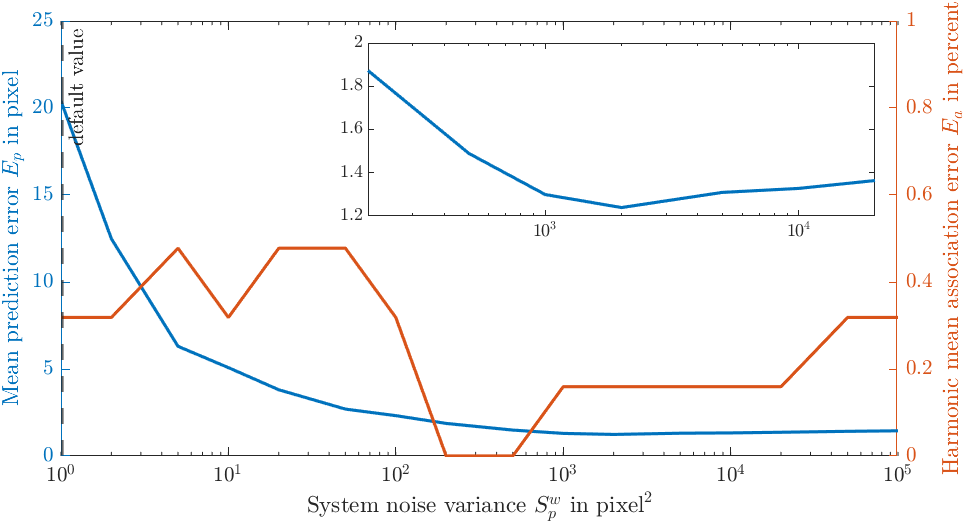
\includegraphics[width=0.9\textwidth]{figures/KF/precov pfeffer cv .png}
\caption{The grid search result of the system noise variance $S^{\boldmath{w}}$ of a peppercorn dataset with the CV model. The small plot shows that the $E_{\mathrm{p}}$ reaches minimum when the $S^{\boldmath{w}}$ is approximately 2,000.}
\label{precov}
\end{figure}

Figures \ref{meacov} and \ref{precov} show the grid search results of the measurement variance $S^{\boldmath{v}}$ and the system noise variance $S^{\boldmath{w}}$ in the CV model. As can be seen in Figure \ref{meacov}, the prediction error was lowered with a lower $S^{\boldmath{v}}$. Figure \ref{precov} shows that a higher $S^{\boldmath{w}}$ also leads to a lower prediction error. The minimized error in both figures is significantly lower than the error with the default hyperparameters. These results suggest a large potentiality for optimization. 

We can make an assumption based on these results. The predictions from the previous steps can be inaccurate because of the difference between the assigned velocity at initialization and the real velocity of the particle, or the difference between the motion model and the real motion of the particle. Thus, the prediction system should use a higher system noise variance to dismiss the error in the previous prediction and a lower measurement variance to keep up with the newest measurement. However, a very high system noise variance means the uncertainty of the previous prediction is very high, and the information contained with the previous prediction is in the update step fully ignored. In this case, the prediction error is heavily affected by the measurement error, which can also cause a higher total error, as shown in the subplot in Figure \ref{precov}. We can observe in that plot that when the system noise variance is about 2,000, the prediction error is minimized. According to the update equation in the Kalman filter, the ratio of the different variances determines the updated value. It means that increasing the $S^{\boldmath{v}}$ has a similar effect of decreasing the $S^{\boldmath{w}}$, when the effects of other hyperparameters are not remarkable. The result of grid search fits this theory well.

% However, when the measurement position error is too low, the change of the prediction error becomes ambiguous. The effects of the different hyperparameters are strongly related, where the final effect depends on the ratio of the hyperparameters. When some of the covariance or variance is too low, it means the certainty of the corresponding variable is very high, and the information contained with other variables is eliminated. In contrast, when some of the covariance or variance is too high, it means the uncertainty of the corresponding variable is very high, and the information contained with the variables is ignored. Therefore, when the hyperparameter is too low or too high, the effect on the prediction error is always not so significant. 

% \textcolor{red}{changed this para}
% With the default association hyperparameters, the association error is higher when the measurement variance is low. As mentioned, when the measurement variance is very low, the prediction error is increased because of the measurement error, which can cause a bad effect on the prediction and the association of the next timestep. However, with a higher $d_{\mathrm{am}}$, which increases the penalty of the new track appearing at middle, the association error is effectively suppressed. The association error stays below 0.5\% with the change of the system noise variance.  

\begin{figure}[htbp]
\centering
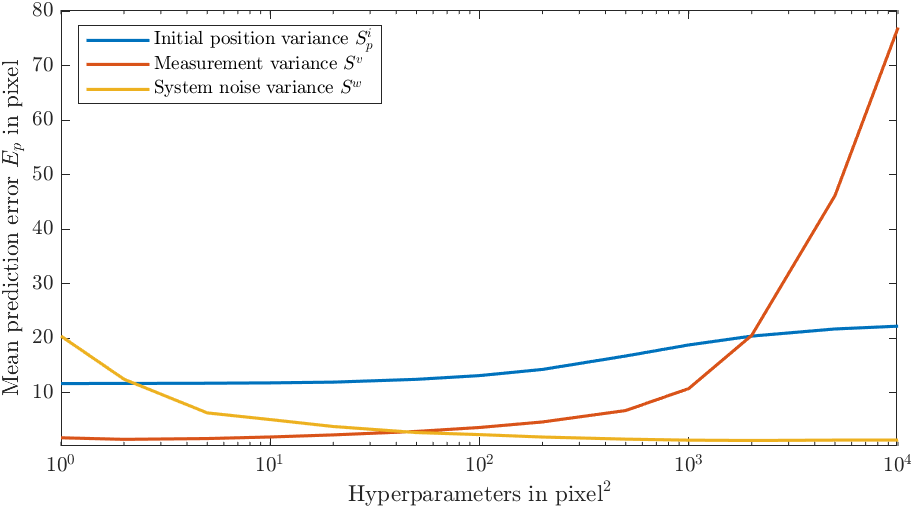
\includegraphics[width=0.8\textwidth]{figures/KF/3cov pfeffer cv.png}
\caption{The grid search result of $S^{i}_{p}$, $S^{\boldmath{v}}$ and $S^{\boldmath{w}}$ of a peppercorn dataset with the CV model.}
\label{3cov}
\end{figure}


Figure \ref{3cov} shows the effect of the initial position variance, measurement variance and system noise variance in the CV model. 
% \textcolor{red}{initial position noise variance, measurement noise variance and prediction noise variance, only the initial one has "position", because the velocity variance is different.}
For each line in this plot, only the mentioned variance is changed and all the other hyperparameters remain as default value. We can see that adjusting the measurement and the system noise variance has a clear effect on the prediction error. Although changing the value of the initial position variance has an effect on the prediction error as well, the effect is not as significant as the other two noise power spectral densities. 

\begin{figure}[htbp]
	\centering
	\begin{subfigure}[t]{0.8\textwidth}
		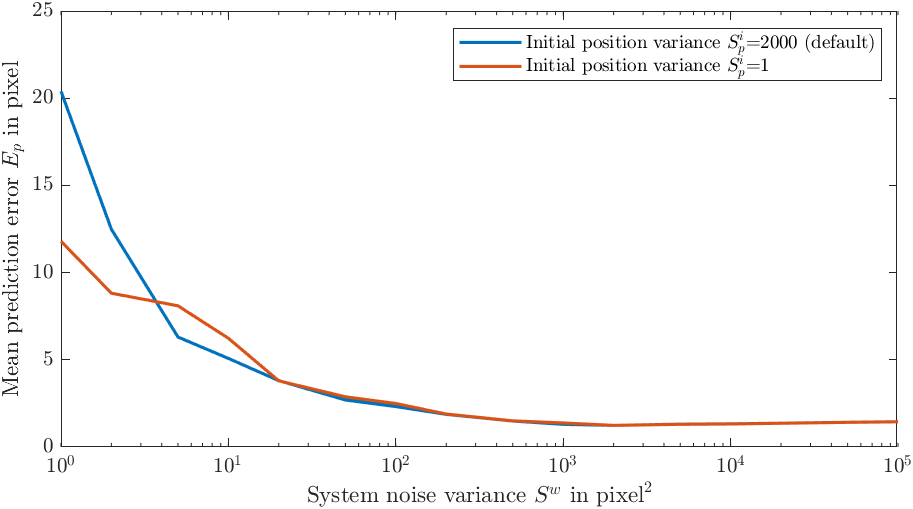
\includegraphics[width=\textwidth]{figures/KF/precov with inicov cv.png}
		\caption{The grid search result of the system noise variance in CV model with varied initial position variance.}
		\label{grid search different default1}
	\end{subfigure}
\end{figure}

\begin{figure}[htbp]
    \ContinuedFloat
    \centering
% 	\vskip\baselineskip
	\begin{subfigure}[t]{0.8\textwidth}
		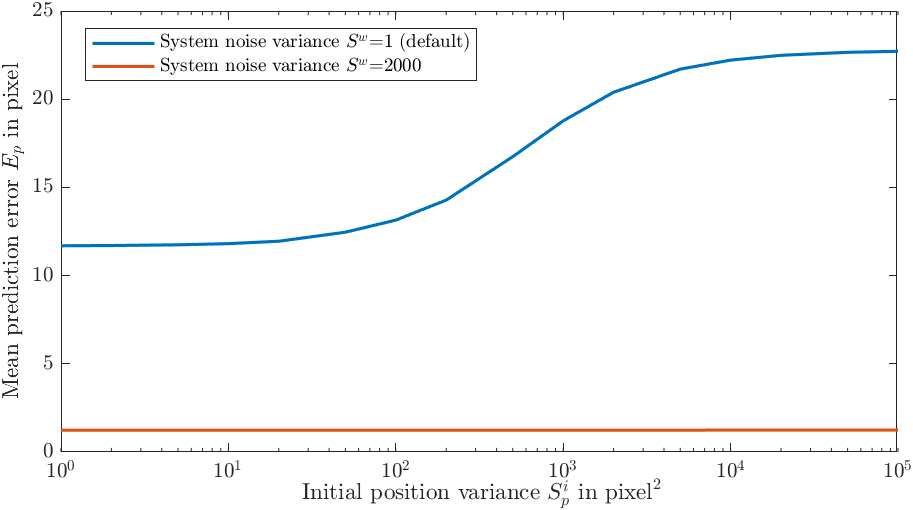
\includegraphics[width=\textwidth]{figures/KF/inicov with precov cv.png}
		\caption{The grid search result of the initial position variance in CV model with varied system noise variance.}
		\label{grid search different default2}
	\end{subfigure}
	\caption{The grid search results of initial position and system noise variance in CV model with only changing these two variance.}
	\label{grid search different default}
\end{figure} 
Figure \ref{grid search different default} presents the grid search results of the initial position and system noise variance in the CV model with varied other variance. In these figures, only the initial position and system noise variance are changed. When the initial position variance is higher, the trend of the prediction error with varied system noise power spectral densities only has a moderate change. But when the system noise variance reaches a high value, the initial position variance has no more effect on the prediction error. It means that the measurement and system noise variance are more valuable to optimize than the initial position variance. After checking the other hyperparameters, as shown in Figure \ref{grid search cv appendix} in Appendix, the measurement and the system noise variance still have the most significant effect on the prediction error in the CV model. Thus, these two hyperparameters are selected for the next step of the optimization.

The result of the CVA model is similar to the CV model. The optimized measurement position variance is lower than the default value, and the optimized prediction position variance is higher than the default. And these two hyperparameters are the most effective hyperparameter among all the hyperparameters for the prediction error. The result is shown in Figure \ref{grid search list} in Appendix. The dataset from each type of the homogeneous material was tested with grid search in both CV and CVA models. The effects of the hyperparameters are similar, which can be seen from Figure \ref{grid search other material} in Appendix. 
% From the the plots the effect of each hyperparameter is clear. We can also find the measurement and system noise variance have the most significant effect on the final tracking error. It should be a important result which is used in the part of optimization. 

\subsubsection{Result of 2-D Grid Search}

% \textcolor{red}{added new section}

Figure \ref{2d cv} shows the test result of a 2-D grid search with the measurement and system noise variance in the CV model. Same as the results from the 1-D grid search, the prediction error is lowered with a lower measurement variance and a higher system noise variance. We can also observe the dark blue area that means the prediction error is minimized. The shape of this area also suggests that the optimized value of the $S^{\boldsymbol{v}}$ and $S^{\boldsymbol{w}}$ should be proportional. The result of the 2-D grid search with the measurement and prediction position variance in the CVA model is illustrated in Figure \ref{2d cva}. A certain area for the optimized hyperparameters is unable to be observed from the plot, but the result still shows that the optimized value of two hyperparameters should be proportional.

\begin{figure}[htbp]
\centering
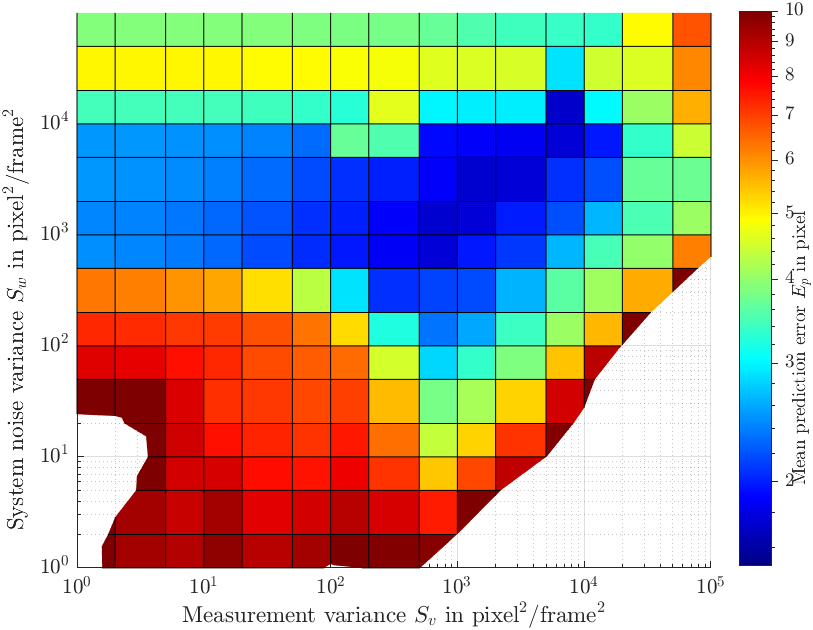
\includegraphics[width=0.8\textwidth]{figures/KF/2d cv1.png}
\caption{The 2-D grid search results of the measurement variance $S^{\boldsymbol{v}}$ and the system noise variance $S^{\boldsymbol{w}}$in the CV model. The data points with the $E_{\mathrm{p}}$ higher than 10 are not shown in this plot.}
\label{2d cv}
\end{figure}

\begin{figure}[htbp]
\centering
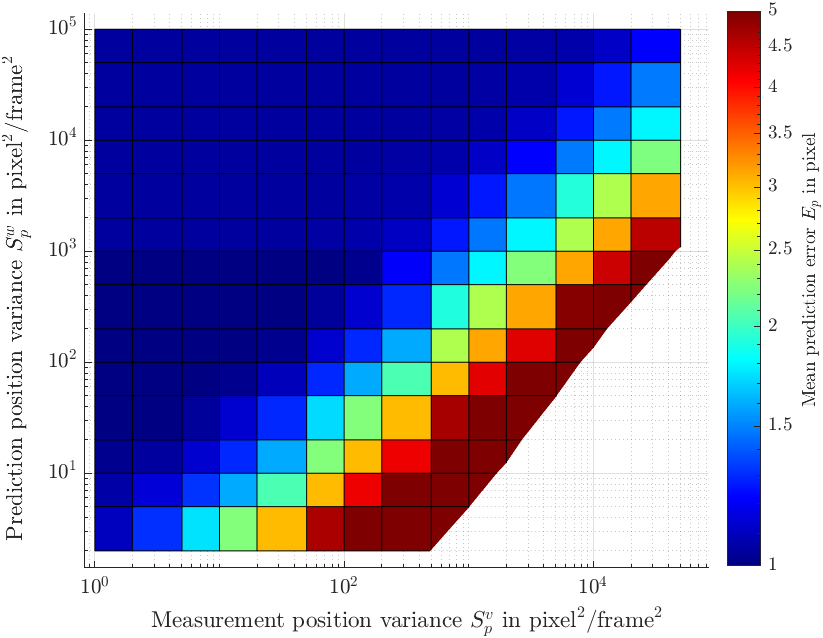
\includegraphics[width=0.8\textwidth]{figures/KF/2d cva1.png}
\caption{The 2-D grid search results of the measurement position variance $S_{\mathrm{pos}}^{\boldsymbol{v}}$ and the prediction position variance $S_{\mathrm{pos}}^{\boldsymbol{w}}$ in the CVA model. The data points with the $E_{\mathrm{p}}$ higher than 10 are not shown in this plot.}
\label{2d cva}
\end{figure}


% \subsubsection{Conclusion}

% From the results above, we can conclude that the prediction error is lower with 

% There should be the plots from 2-3 sets of hyperparameters in both CV and CVA model, e.g. measurement position covariance and initial position covariance. The main aim of this part is to show the different effect when two hyperparameter change at the same time. One hyperparameter should have more effect than the other one, so we can find the difference of the "important" and "unimportant" hyperparameters raised in the last section.

% \FloatBarrier

% \subsection{Results of Bayesian Optimization}

\subsection{Validation of the Bayesian Optimization Method}
\label{validation}
% Give some introduction of generating datasets. 
% Add a table of some experiment results of the generated datasets. The results from the optimization is very similar from the real parameters, showing the optimization method can reconstruct the real hyperparameters of the system.

In order to confirm the validity of the Bayesian optimization method, the implemented optimization algorithm was first tested with artificial datasets. During the optimization, only one or two hyperparameters were optimized at the same time, and the other hyperparameters kept the same value with the setting for generating the dataset. When the optimized values of the hyperparameters are the same as the value in the setting, the optimization algorithm can be recognized to be able to reconstruct the hyperparameters in the system.

% To overcome the interference of the random noise, the optimization for each hyperparameter was done with ten datasets under the same settings, as mentioned in \Sec{Artificial Datasets}. The final optimization result is the average value of the optimized result from all datasets.

The result of the optimized hyperparameters and the original hyperparameters from the dataset are presented in Table \ref{validationHPs} and \ref{validationHPs2d}. The difference between the value of the hyperparameters given in the dataset generation and the value of the optimized hyperparameters is lower than 1\% on average. These results suggest that the Bayesian optimization method can reconstruct the real hyperparameters of the system. 

\begin{table}[htbp] 
    % \small
    \centering
    \caption{Optimized hyperparameters and the original hyperparameters from the dataset in the validation dataset in 1-D Bayesian optimization. The original and optimized values are similar, which suggests that the Bayesian optimization method is able to reconstruct the hyperparameters in a dynamic system.} 
    \begin{tabular}{cccc} 
    \toprule 
    \multirow{2}*{Model}&\multirow{2}*{Hyperparameters}&Original &Optimized \\ 
         &               &value&value\\ 
    \midrule 
    \multirow{3}*{CV}&Measurement variance  $S^{\boldsymbol{v}}$&0.1&0.10020\\
     &System noise variance $S^{\boldsymbol{w}}$&0.1&0.10045\\
     &Initial velocity $v_{0}$&100&100.01\\
    \multirow{4}*{CVA}&Measurement position variance $S_{\mathrm{pos}}^{\boldsymbol{v}}$  &0.1&0.10081\\
     &Prediction position variance $S_{\mathrm{pos}}^{\boldsymbol{w}}$&0.1&0.09820\\ 
     &Measurement velocity variance $S_{\mathrm{vel}}^{\boldsymbol{v}}$&0.1&0.09923\\ 
     &Initial velocity $v_{0}$&100&100.02\\
    \bottomrule 
    \end{tabular} 
    \label{validationHPs}
\end{table}

\begin{table}[htbp] 
    % \small
    \centering
    \caption{Optimized hyperparameters and the original hyperparameters from the dataset in the validation dataset in 2-D Bayesian optimization. The original and optimized values are similar, which suggests that the Bayesian optimization method is able to reconstruct the hyperparameters in a dynamic system.} 
    \begin{tabular}{cccc} 
    \toprule 
    \multirow{2}*{Model}&\multirow{2}*{Hyperparameters}&Original &Optimized \\ 
         &               &value&value\\ 
    \midrule 
    \multirow{2}*{CV}&Measurement variance  $S^{\boldsymbol{v}}$&0.1&0.10071\\
     &System noise variance $S^{\boldsymbol{w}}$&0.1&0.09898\\
    \multirow{2}*{CVA}&Measurement position variance $S_{\mathrm{pos}}^{\boldsymbol{v}}$  &0.1&0.10145\\
     &Prediction position variance $S_{\mathrm{pos}}^{\boldsymbol{w}}$&0.1&0.09912\\
    \bottomrule 
    \end{tabular} 
    \label{validationHPs2d}
\end{table}



However, we only tested the case, where the motion of the particles follows exactly the motion model. The effect of the difference between the real motion and the motion models on the hyperparameter is not examined. These effects are hard to express with the functions of the hyperparameters. Therefore, we are unable to check this effect with the artificial data with the method in this section.

\subsection{Results of Bayesian Optimization on the Peppercorn Dataset}
\label{Tests of Bayesian Optimization}
\subsubsection{Results of Bayesian Optimization in Higher Dimension}

In \Sec{1d}, the most effective hyperparameters for both motion models were given. In this section, these hyperparameters were optimized with the Bayesian optimization algorithm. According to the update equation in the Kalman filter, the ratio of the different variances determines the updated value. The 2-D optimization result presented in Figure \ref{opt 2d} also shows that the optimized values of the two hyperparameters are proportional. This feature enables us to operate the optimization with only one hyperparameter. Thus, the search space for optimization is reduced, which can increase the accuracy and efficiency of the optimization.
% \textcolor{red}{the algorithm converges faster when optimizing only 1 HP.} 

\begin{figure}[htbp]
\centering
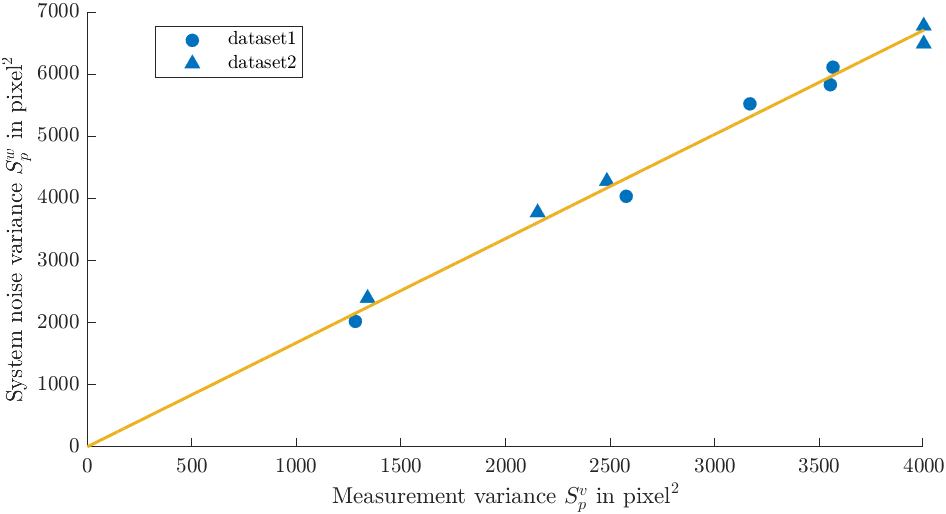
\includegraphics[width=0.7\textwidth]{figures/KF/bayopt/opt 2d cv.png}
\caption{The result of the 2-D optimization of $S^{\boldsymbol{v}}$ and $S^{\boldsymbol{w}}$ with two peppercorn datasets. The optimized values of the two hyperparameters are proportional.}
\label{opt 2d}
\end{figure}

\begin{figure}[htbp]
\centering
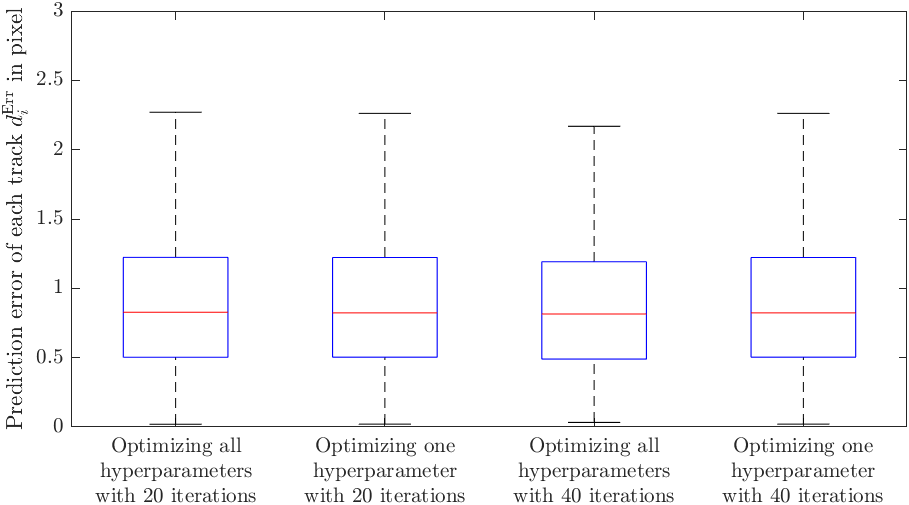
\includegraphics[width=0.7\textwidth]{figures/KF/bayopt/effect opt all.png}
\caption{The comparison of the 5-D optimization result of all hyperparameters in CV model and the 1-D optimization result of $S^{\boldsymbol{w}}$ with a peppercorn datasets. }
\label{opt 5d}
\end{figure}

Figure \ref{opt 5d} shows the comparison of the 5-D optimization result of all hyperparameters in the CV model and the 1-D optimization result of $S^{\boldsymbol{w}}$ with a peppercorn dataset. We can observe that the prediction error from the 1-D optimization is very similar to the prediction error from the 5-D optimization. And the difference from the prediction error with different iterations is also not significant. Therefore, using the 1-D Bayesian optimization with 20 iterations is enough to obtain satisfactory results on the optimized hyperparameters. Based on these results, we can confirm that the 1-D Bayesian optimization can archive a similar effect as the optimization with higher dimensions. Therefore, in the following sections we are using the 1-D Bayesian optimization.   



% We find first that when we optimizing two hyperparameters at the same time, the two optimized hyperparameters are proportional. It shows that the effect of the other HPs are less. That also enables us to operate the optimization with only one HP, which can increase the accuracy and the efficiency of the optimization.

% Some optimization results with different models (CV and CVA) and different datasets (sphere, cylinder, cuboid and pepper).

\subsubsection{Results of 1-D Bayesian Optimization}

In the following sections, only the system noise variance $S^{\boldsymbol{w}}$ in the CV model and the prediction position noise power spectral density $S_{\mathrm{pos}}^{\boldsymbol{w}}$ in the CVA model is optimized, and the other hyperparameters remain the default values. Figure \ref{opt cv sph} shows an intermediate result of the Bayesian optimization of a sphere dataset with the CV model. The algorithm constructs a surrogate model for the prediction error.

\begin{figure}[htbp]
\centering
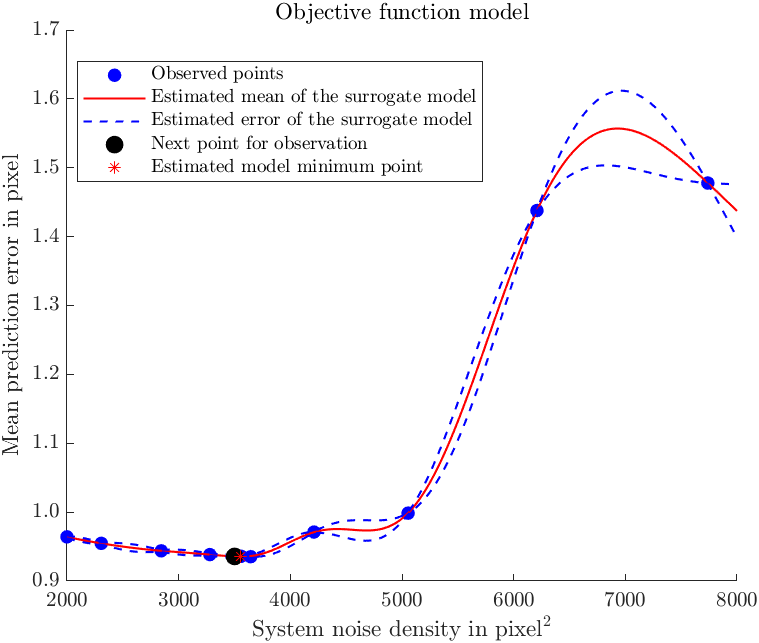
\includegraphics[width=0.6\textwidth]{figures/KF/bayopt/bayopt line pfeffer.png}
\caption{The intermediate result of the Bayesian optimization of a peppercorn dataset with the CV model.}
\label{opt cv sph}
\end{figure}

In Figures \ref{opt effect1} and \ref{opt effect2} the effect of the optimization is visualized with box plots. The plots present the distribution of the prediction errors of all tracks in the peppercorn dataset for test. The upper and lower bound of the boxes in the box indicate respectively the upper quartile $Q_{3}$ and lower quartile $Q_{1}$ of the errors, and the red line in the middle of boxes represents the median of the errors. The maximum length of the whiskers is determined as $1.5(Q_{3}-Q_{1})$. The outliers are not shown in the plots.


From the box plots, we can observe that the accuracy of the prediction with optimized hyperparameters is significantly higher than with the default hyperparameters. The prediction error with optimized hyperparameters is also approximately 10\% lower than the results from Hornberger \cite{hornberger2018} in the CV model. The association error with the optimized hyperparameters is limited in an acceptable range, which is less than 1\% in each dataset.

In Table \ref{opt pfeffer}, the optimized values of the hyperparameters from grid search have a significant difference from the results from Bayesian optimization because of high step size. The results with the hyperparameters from Bayesian optimization are also slightly better than the results from grid search. Because of the settings of the grid points, grid search is not always able to find the optimized value for the hyperparameters. Although employing a smaller step size can increase the possibility of finding the optimized value, the computation need is also increasing. In this respect, Bayesian optimization is a more efficient method for hyperparameter optimization.





\begin{table}[htbp] 
\small
    \centering
    \caption{List of the default and optimized value of the $S^{\boldsymbol{w}}$ in the CV model and $S_{\mathrm{pos}}^{\boldsymbol{w}}$ in the CVA model for the peppercorn dataset.} 
    \begin{tabular}{ccc} 
    \toprule 
    Hyperparameters &Optimization method  &Value\\ 
    \midrule 
    \multirow{3}*{$S^{\boldsymbol{w}}$}&  Default   &1\\
    &Optimized with grid search                     &2000\\
    &Optimized with Bayesian optimization           &3508.1\\
    \multirow{3}*{$S_{\mathrm{pos}}^{\boldsymbol{w}}$}&Default &16.7\\
    &Optimized with grid search                     &20000\\
    &Optimized with Bayesian optimization           &20301\\
    \bottomrule 
    \end{tabular} 
    \label{opt pfeffer}
\end{table}

\begin{figure}[htbp]
\centering
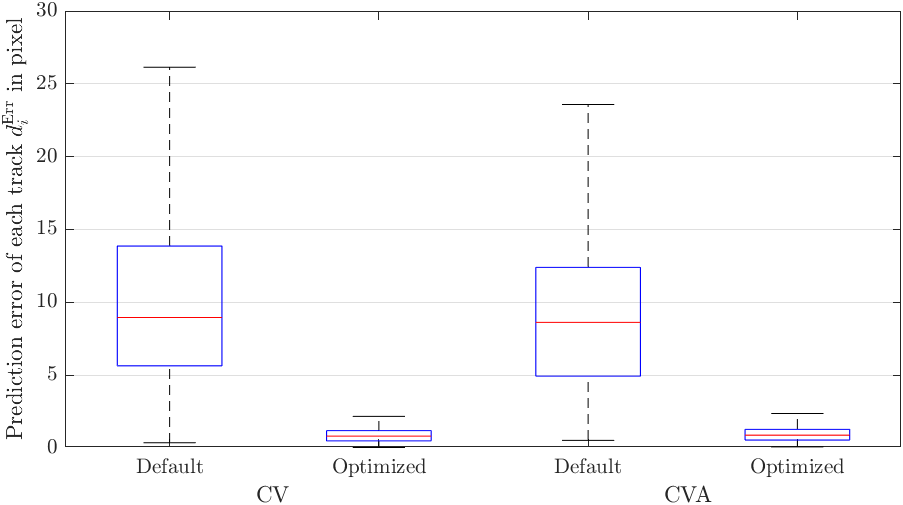
\includegraphics[width=0.7\textwidth]{figures/KF/bayopt/effect opt4.png}
\caption{Comparison of the prediction error with the default and optimized hyperparameters with the peppercorn datasets.}
\label{opt effect1}
\end{figure}

\begin{figure}[htbp]
\centering
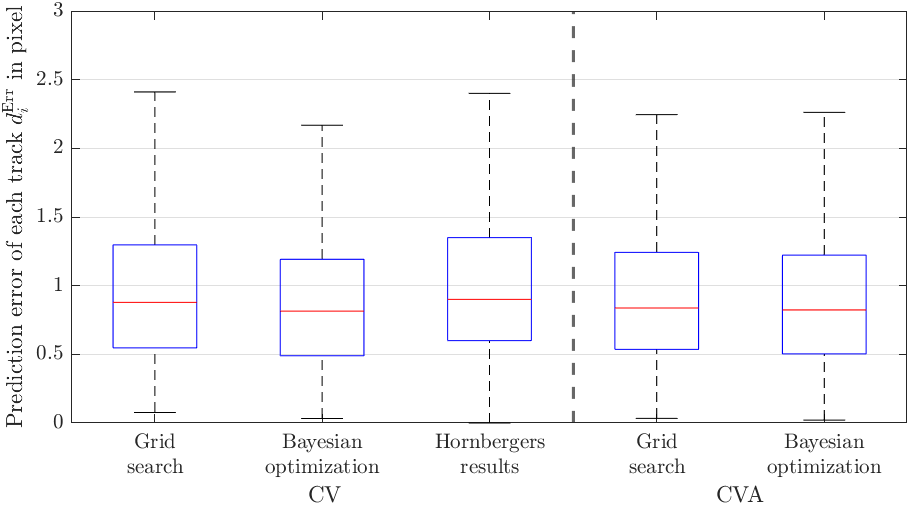
\includegraphics[width=0.8\textwidth]{figures/KF/bayopt/effect opt3.png}
\caption{Comparison of the prediction error with the hyperparameters from different optimization methods with the peppercorn datasets.}
\label{opt effect2}
\end{figure}

% \subsection{Clustering and Mapping}
\subsection{Results of Bayesian Optimization with Different Materials}
\label{Test of Different Materials}
\subsubsection{Results of Homogeneous Materials}
% Try to make clusters between different datasets. Make plots showing results from different datasets. The results from different datasets are similar within the same datasets and different between different datasets, showing the different materials applies for different hyperparameters. After that give some analysis or assumption of the reason causing these difference between the datasets. 

Figures \ref{cluster1} and \ref{cluster2} present the optimized values of the system noise variance in the CV model and the system position noise power spectral density in the CVA model for varied materials.
% \textcolor{red}{You highlighted here. Is that too long?} 
It can be seen from the optimization result that different materials have different ranges of optimized hyperparameters. The comparison of the prediction error between different optimization methods of each material is presented in Figure \ref{effect opt appendix} in Appendix.

The difference between the optimized hyperparameters comes primarily from the difference in the motion characteristics of the different types of materials. For example, the spheres are easy to roll on the conveyor belt, but the cylinders can roll only when the particle lies in a specific direction. That means the velocities of spheres are more likely to be different from the belt velocity than cylinders. These characteristics make the real motion of the particles different from the motion model, and this difference needs to be compensated from the noise term in the motion model. Therefore, the different values of the hyperparameters that represent the different system and measurement noise power spectral densities should be applied to different types of materials.

\begin{figure}[htb]
\centering
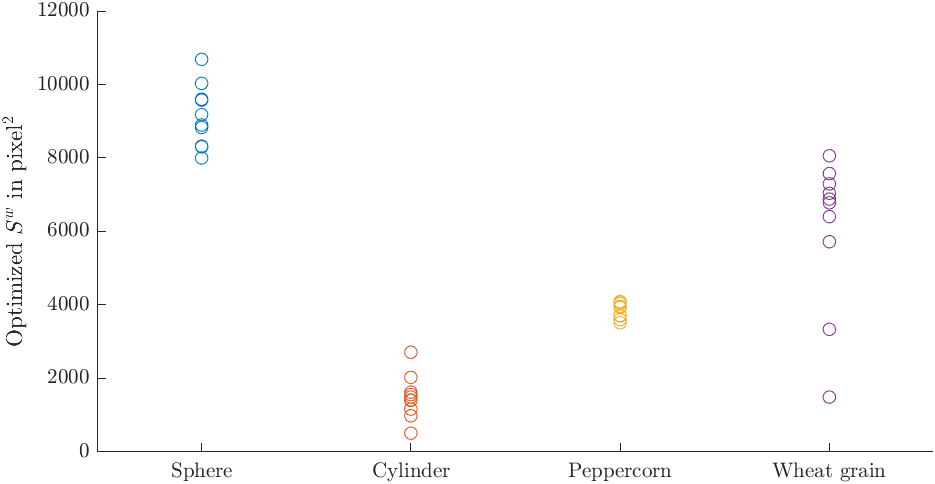
\includegraphics[width=0.7\textwidth]{figures/KF/bayopt/opt all CV.png}
\caption{The optimized value of the system noise variance in CV model for different materials.}
\label{cluster1}
\end{figure}

\begin{figure}[htb]
\centering
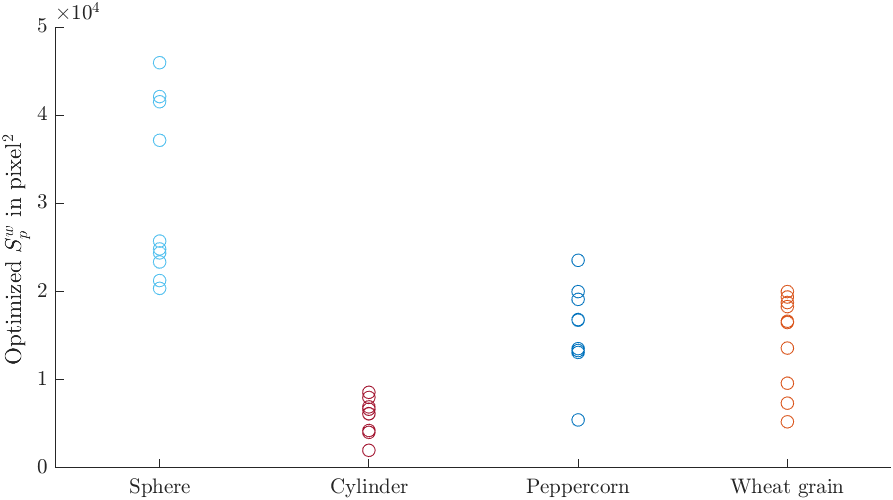
\includegraphics[width=0.7\textwidth]{figures/KF/bayopt/opt all CVA.png}
\caption{The optimized value of the system position noise power spectral density in CVA model for different materials.}
\label{cluster2}
\end{figure}

However, the optimized values of the hyperparameters are distributed in a wide range, and the range of the hyperparameters of various materials often overlaps from each other. For example, the range for the peppercorn and the wheat grain is very similar in Figure \ref{cluster2}. It makes the clustering work more challenging. This phenomenon is possibly due to the ``flat area" in the hyperparameter space. As shown in Figure \ref{precov}, the error in a wide range around the optimal value of the hyperparameter remains almost the same. It means a slight random error in the tracking process can cause a remarkable difference in the optimization result. The wide distribution of the optimized hyperparameters can also attribute to some other differences between datasets, such as the density of the particles on the belt.


\FloatBarrier

\subsubsection{Results of Mixed Materials}


Table \ref{resultmix} presents the result of the optimized value of the $S^{\boldsymbol{w}}$ and $S_{\mathrm{pos}}^{\boldsymbol{w}}$ for the mixture materials dataset. We observed that the optimized $S^{\boldsymbol{w}}$ and $S_{\mathrm{pos}}^{\boldsymbol{w}}$ here is much lower than the value from the homogeneous materials. 

The shape and size features can have an effect on the measurement noise. The particle size in the mixture varies dramatically, while the size of homogeneous materials is the same within a dataset. The shapes of the mixture materials are also irregular. These characteristics increase the hurdles of detecting the midpoint location of the particles, which also increases the measurement noise. Because of the high noise, the track results are heavily affected by the random factors, which causes the optimized hyperparameters in different datasets distributed in a wide range. The comparison of the prediction errors with the default and optimized hyperparameters with the mixed material datasets.

\begin{table}[htbp] 
\centering
\caption{List of the optimized value of the $S^{\boldsymbol{w}}$ and $S_{\mathrm{pos}}^{\boldsymbol{w}}$ for the mixture materials dataset.} \small
\begin{tabular}{ccc} 
\toprule 
Hyperparameters &Dataset &Value\\ 
\midrule 
\multirow{3}*{$S^{\boldsymbol{w}}$}& 1 &9609.8\\
&2 &2350.1\\
&3 &570.6\\
\multirow{3}*{$S_{\mathrm{pos}}^{\boldsymbol{w}}$}&1 &15227.3\\
&2 &2104.8\\
&3 &4136.3\\
\bottomrule 
\end{tabular} 
\label{resultmix}
\end{table}

\FloatBarrier

\section{Robust Range of Association Hyperparameters}
\label{Robust Range of Association Hyperparameters}

\subsection{Results with Grid Search}

\begin{figure}[htb]
\centering
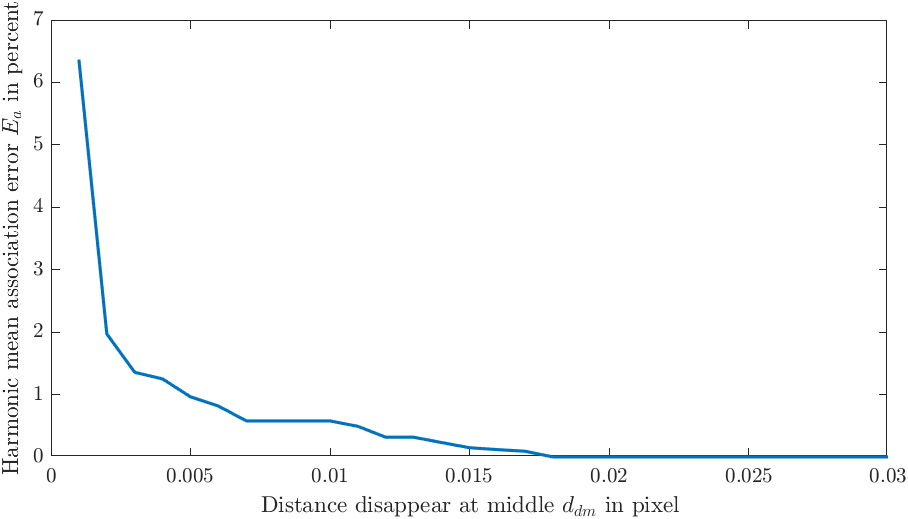
\includegraphics[width=0.8\textwidth]{figures/Asso/gridsearch1.png}
\caption{The grid search result of the distance disappear at middle $d_{\mathrm{dm}}$ on the association error with the DEM dataset.}
\label{asso gs1}
\end{figure}

\begin{figure}[htb]
\centering
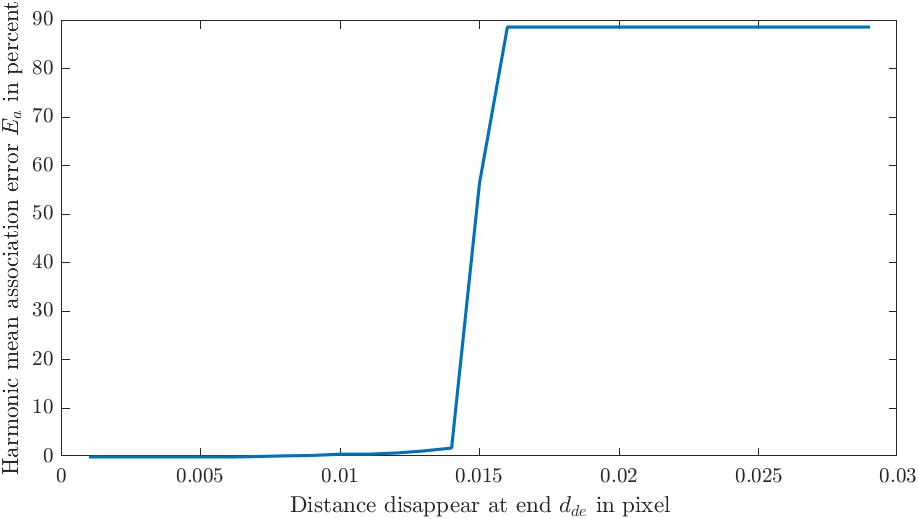
\includegraphics[width=0.8\textwidth]{figures/Asso/gridsearch2.png}
\caption{The grid search result of the distance disappear at end $d_{\mathrm{de}}$ on the association error with the DEM dataset.}
\label{asso gs2}
\end{figure}

The effects of the association hyperparameters are first tested with grid search on the DEM dataset. Figures \ref{asso gs1} and \ref{asso gs2} reveal the effect of the distance disappear at middle $d_{\mathrm{dm}}$ and the distance disappear at end $d_{\mathrm{de}}$ on the association error. According to Figure \ref{asso gs1}, the tracking results have no association error as the $d_{\mathrm{dm}}$ is higher than 0.018. Therefore, the range above 0.018 can be considered as the robust range for $d_{\mathrm{dm}}$. However, when the distance decreases lower than 0.018, the association error begins to increase slightly. When the distance is more close to zero, the association error increases more sharply. The distance disappear at end has a robust range below 0.005, as shown in Figure \ref{asso gs2}. The association error grows steadily with the increase of the distance lower than 0.014, and then have a steep increase between 0.014 and 0.016. After that, the association error reaches nearly 90\%, which indicates the tracking algorithm is unable to provide a reasonable association in this range. These results are easy to understand qualitatively: a particle is less possible to leave the tracking area at the middle of the area, but more possible to leave at the end phase. Therefore, the distance disappear at middle should be higher, and the distance disappear at end should be generally low. The effect of the other hyperparameters is also examined with the same method, and the results are presented in Figure \ref{grid search other} in Appendix.

% Similar to the part of the prediction hyperparameters, each association  hyperparameter is also tested with the grid-search-like method, in order to find the effect of each hyperparameter on the association error.

% ...The distance ...should be higher....and ... should be lower....


% \FloatBarrier


\subsection{Results with SVM}

% (Results with SVM)
% Several plots like this. After plots give some analyze ().

After the grid search, some SVMs were trained with the training dataset mentioned in \Sec{training data svm}. The SVMs present the range of the association hyperparameters with no association hyperparameters. This range can represent the robust range of the association hyperparameters.

Some results of the robust range acquired from two-dimensional SVMs are depicted in Figures \ref{svm1} and \ref{svm2}. In Figure \ref{svm1} we can observe that the robust range of the distance disappear at middle $d_{\mathrm{dm}}$ is roughly above 0.018, which meets the result from the grid search. The lower bound of the distance appear at middle $d_{\mathrm{am}}$ is unable to see from the plot. We can make an assumption that the lower bound of the distance appear at middle could be lower than zero. However, we can still notice that when the $d_{\mathrm{dm}}$ is close to zero, the lower bound for the robust range of the $d_{\mathrm{am}}$ increases to 0.02. It means there is still a correlation between the value and the robust range of the two hyperparameters.

\begin{figure}[htb]
\centering
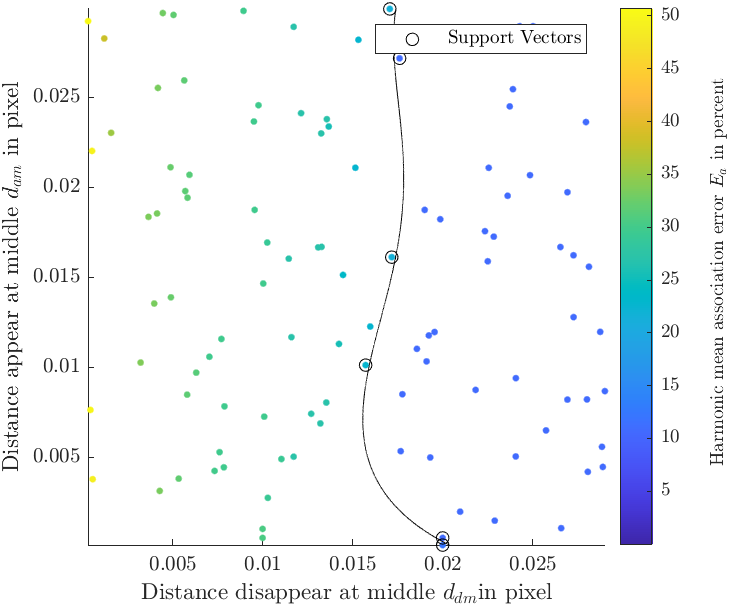
\includegraphics[width=0.6\textwidth]{figures/Asso/overfitting2.png}
\caption{The 2-D SVM result of the distance disappear at middle and the distance appear at middle with DEM dataset.}
\label{svm1}
\end{figure}

Figure \ref{svm2} shows the robust range of the distance disappear at middle and the distance no change. It is obvious that the lower bound for the distance disappear at middle $d_{\mathrm{dm}}$ is strongly related to the value of the distance no change $d_{\mathrm{n}}$. Recalling the example raised in \Sec{Robust Range of the Association Hyperparameters}, the results shown in two figures conform to the theoretical analysis of the robust range. When the distance no change is higher, the sum of the distance disappear at middle and the distance appear at middle should be also higher for a correct association.

\begin{figure}[htb]
\centering
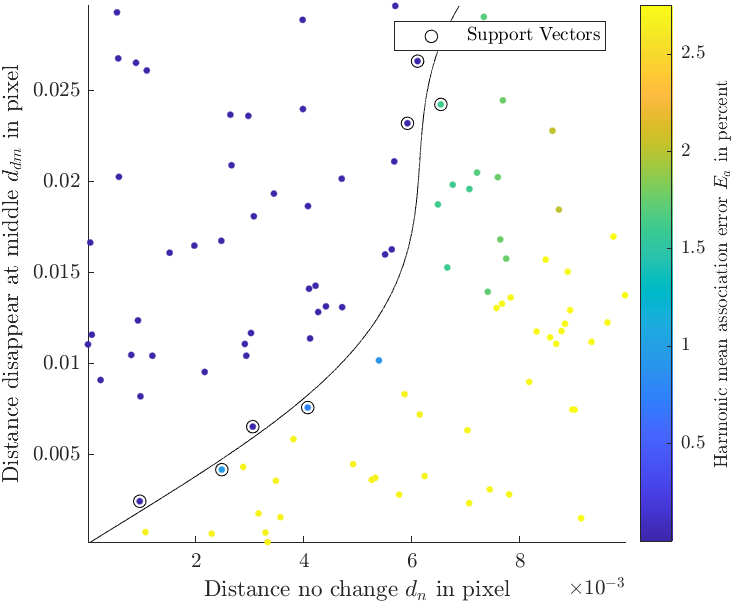
\includegraphics[width=0.6\textwidth]{figures/Asso/2d svm.png}
\caption{The 2-D SVM result of the distance no change and the distance appear at middle with DEM dataset.}
\label{svm2}
\end{figure}

\begin{figure}[htb]
\centering
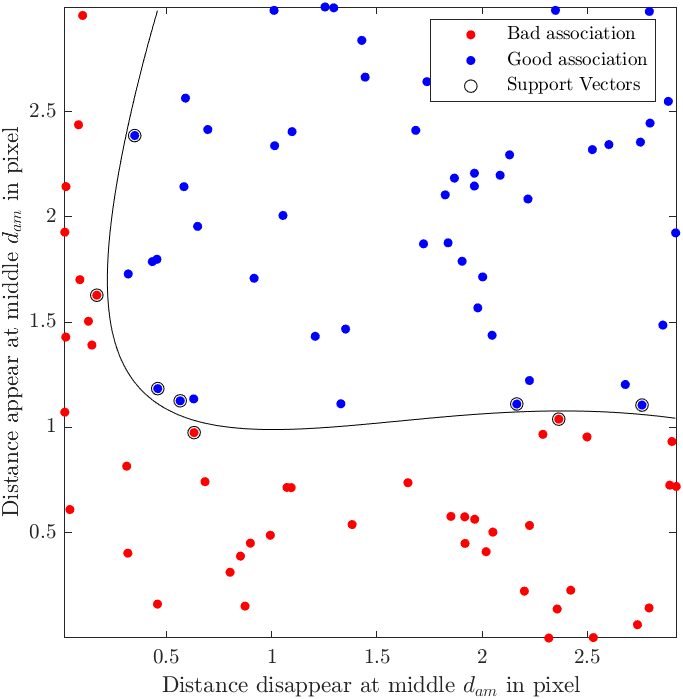
\includegraphics[width=0.5\textwidth,height=0.5\textwidth]{figures/Asso/2d svm sphere.png}
\caption{The two dimensional SVM result of the distance disappear at middle and the distance appear at middle with the sphere dataset.}
\label{svm3}
\end{figure}

However, the robust range of association hyperparameters for different datasets can be very different. In Figure \ref{svm3}, the lower bound for the distance appear at middle $d_{\mathrm{am}}$ for the sphere dataset is about two. Since the tracking error of the different datasets is different, the association hyperparameters should be certainly different. Therefore, the robust range of association hyperparameters for different datasets should be determined separately. However, the datasets that have similar tracking errors are acceptable to take the same robust range of association hyperparameters. For example, all the experiments on the hyperparameters for motion prediction with real datasets are performed with the same association hyperparameters.


The shape of the boundary curve of the robust range for the sphere dataset is similar to the DEM dataset. It suggests that the reasons for those curve shape for different materials are also similar. These reasons are explained in the next section.

In order to determine the robust range in a higher-dimensional space, the SVMs were also trained with varying all the five association hyperparameters. To examine the accuracy of the trained SVMs, the SVM classifiers were tested with the test dataset. The test result is shown in Table \ref{svm test}. It shows that the SVM classifiers have obtained a satisfactory classification accuracy. The decision boundary in the 3-D space is shown in Figure \ref{3d svm}.


\begin{table}[htb] 
    \centering
    \caption{Classification accuracy of the SVM classifiers on the test dataset.} 
    \begin{tabular}{ccc} 
    \toprule 
     & Classified as & Classified as\\ 
     & with association errors & no association errors\\
    \midrule 
    with association errors & 500 &14 \\
    no association errors   & 3  &483 \\
    \bottomrule 
    \end{tabular} 
    \label{svm test}
\end{table}



\begin{figure}[htbp]
\centering
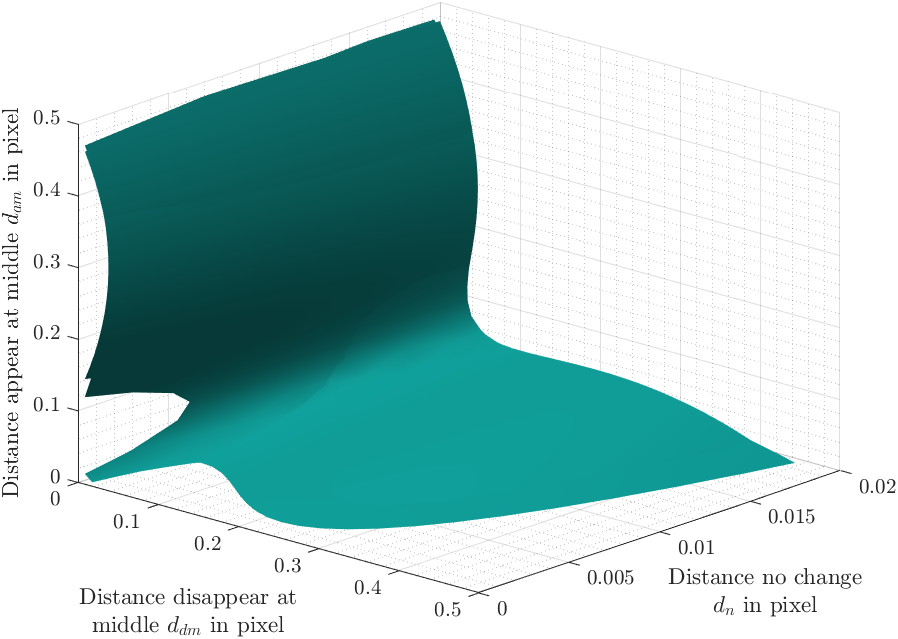
\includegraphics[width=0.7\textwidth]{figures/Asso/3d svm.png}
\caption{The decision boundary of the SVM in 3-D space.}
\label{3d svm}
\end{figure}


\FloatBarrier

\subsection{Analysis of the Robust Range of the Association Hyperparameters}

% \textcolor{red}{write something about the effect of the hyperparameters. How it controls the association. Why some should low and why should some high}

Considering only the association error caused by inappropriate association hyperparameters, the error can be divided into two types, as illustrated in Figure \ref{association error example}. The first type is that a single track is separated into two tracks in the middle. When the distance no change is too high or the other distance is too low, this error happens. Take the association matrix in Figure \ref{asso example simple} as an example, when the summation of the distance between the prediction and the new measurements, as the left above block, and the distance no change is higher than the summation of the other two distances, the GNN algorithm would choose the left below and the right above blocks, which means there is a track with no assigned measurements and a new track. To avoid this error, the distance no change should have an upper bound, and the other distances should have a lower bound. The upper and lower bound here are strongly related. This result can also explain the reason for the boundary shape of the robust ranges shown in Figures \ref{svm1}, \ref{svm2} and \ref{svm3}.

\begin{figure}[htbp]
\centering
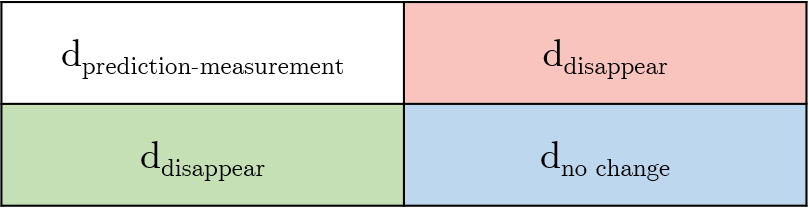
\includegraphics[width=0.6\textwidth]{figures/Asso/association matrix example simple.png}
\caption{A simple example of the association matrix.}
\label{asso example simple}
\end{figure}

We take the maximum Mahalanobis prediction error $d_{\mathrm{pre-mea}}^{\mathrm{max}}$ representing the maximum Mahalanobis distance between associated predictions and measurements. In order to avoid the type of error mentioned above, we propose that the summation of the distance for appearing and disappearing should be lower than the summation of the $d_{\mathrm{pre-mea}}^{\mathrm{max}}$ and the distance no change $d_{\mathrm{n}}$. Therefore, the value of the hyperparameters follows these inequalities
\begin{equation}\label{assoeq1}
    d_{\mathrm{n}} + d_{\mathrm{pre-mea}}^{\mathrm{max}} \leqslant 
    \left\{
         \begin{array}{ll}
         d_{\mathrm{as}} + d_{\mathrm{dm}}, \quad&\textrm{for start phase}\\
         d_{\mathrm{am}} + d_{\mathrm{dm}}, \quad&\textrm{for middle phase}\\
         d_{\mathrm{am}} + d_{\mathrm{de}}, \quad&\textrm{for end phase}  
         \end{array}
    \right . 
\end{equation}

After manual checks, all the default values of the association hyperparameter for both real and DEM datasets are in the robust range. The $d_{\mathrm{pre-mea}}^{\mathrm{max}}$ in the DEM dataset with default hyperparameters is about $0.05$ m. The $d_{\mathrm{pre-mea}}^{\mathrm{max}}$ in the peppercorn dataset is about $0.35$ pixel with the default prediction hyperparameter. Therefore, the default hyperparameters fit in  Inequality \eqref{assoeq1}. A lower measurement covariance can increase the Mahalanobis distance. Because of this effect, the $d_{\mathrm{am}}$ is set higher as the default value when the measurement noise power spectral density is set at a low value.
% \textcolor{red}{since the default value is robust, I'm not going to do more other tests on the real datasets.}

\begin{figure}[htbp]
	\centering
	\begin{subfigure}[t]{0.3\textwidth}
		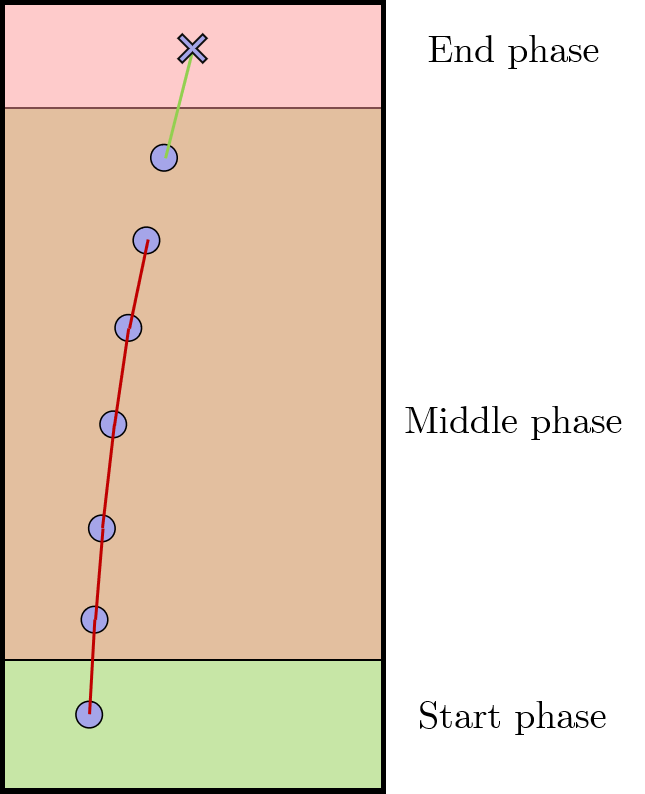
\includegraphics[width=\textwidth]{figures/Asso/association error example1.png}
		\caption{An association error occurred because a single track is separated into two tracks in the middle of the track.}
	\end{subfigure}
	\quad
	\begin{subfigure}[t]{0.3\textwidth}
		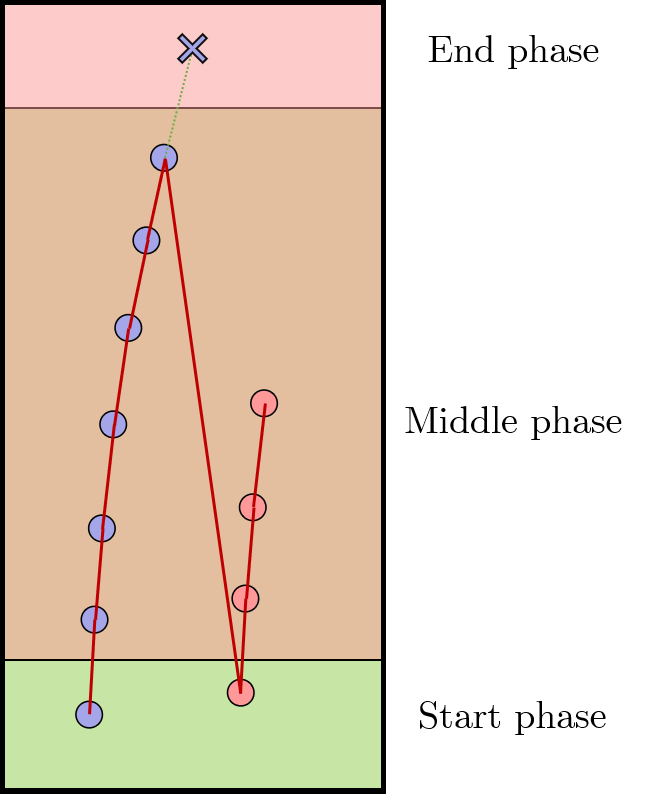
\includegraphics[width=\textwidth]{figures/Asso/association error example2.png}
		\caption{An association error occurred because a track can not end properly.}
	\end{subfigure}
	\caption{Two types of association errors caused by inappropriate association hyperparameters.}
	\label{association error example}
\end{figure}



Another type is that a track can not end properly. It means this track is not considered as ended when it reaches the end but assigned with a new appeared measurement. When the track disappears in the middle of the observation area, this type of error does not affect the final separation accuracy, since the number of tracks reaching the end of the observation area remains unchanged. However, when the track disappears in the end, this type of error will produce some tracks that contain only one or two measurements, which usually have a high prediction error. This type often happens when the distance disappear at end and the distance appear at start is too high, such as the area over 0.015 in Figure \ref{asso gs2}, because the tracks are mainly appearing at the start phase and disappearing in the end phase. However, when the datasets contain the tracks that should appear and disappear in the middle, the corresponding hyperparameters should have also a limited upper bound.

The distance between measurements and the other the predictions from other tracks $d_{\mathrm{other}}$ are introduced for explaining this type of error. Considering only the track reaches the end phase when the track is associated with a measurement not belonging to other tracks, the inequalities are presented as 
\begin{equation}
    \label{assoeq2}
    d_{\mathrm{other}} + d_{\mathrm{n}}\geqslant\  
    \left \{
    \begin{array}{ll}
    d_{\mathrm{am}} + d_{\mathrm{de}} ,\quad&\textrm{for the measurement in start phase}\\ 
    d_{\mathrm{as}} + d_{\mathrm{de}} ,\quad&\textrm{for the measurement in middle or end phase}
    \end{array}.  
    \right.  
\end{equation}
And when the associated measurement belongs to another existing track $i$, the inequalition is presented as
\begin{equation}
    d_{\mathrm{de}} + d_{i}^{\mathrm{Err}} \leqslant\  d_{\mathrm{other}} + d_{\mathrm{n}}.
    \label{assoeq3}
\end{equation}
These inequalities determine the upper bound of the $d_{\mathrm{de}}$, $d_{\mathrm{am}}$ and $d_{\mathrm{as}}$. The $d_{\mathrm{other}}$ is determined by the local density of the particles. Therefore, even if the overall density is low, the $d_{other}$ can be in some position high. However, the $d_{other}$ is determined by the overall density of particles on the belt in general.

From the analysis above, the robust range is greatly influenced by the average prediction error. Therefore, the quality of the motion prediction also causes a massive effect on the robust range of the association hyperparameters. When the prediction is more accurate, the association hyperparameters can allow a wider robust range without increasing the association error.

Theoretically, all the association hyperparameters should have a lower bound and an upper bound. However, in our search, there are some hyperparameters having a lower bound below than zero. A negative distance is out of the domain of definition. Therefore, the lower bound for the robust range is defined as zero in this case.


\begin{table}[htbp] 
    % \small
    \centering
    \caption{Two test sets of the robust and unrobust association hyperparameters for the peppercorn dataset.} 
    \begin{tabular}{ccc} 
    \toprule 
    Settings&Hyperparameters& Value\\ 
    \midrule 
    \multirow{5}*{Robust}&Distance appear at start $d_{\mathrm{as}}$&0.1\\
    &Distance appear at middle $d_{\mathrm{am}}$&0.18\\
    &Distance disappear at end $d_{\mathrm{de}}$&0.1\\
    &Distance disappear at middle $d_{\mathrm{dm}}$&0.18\\
    &Distance no change $d_{\mathrm{n}}$&0\\
    ~\\
    \multirow{5}*{Unrobust}&Distance appear at start $d_{\mathrm{as}}$&0.1\\
    &Distance appear at middle $d_{\mathrm{am}}$&0.15\\
    &Distance disappear at end $d_{\mathrm{de}}$&0.1\\
    &Distance disappear at middle $d_{\mathrm{dm}}$&0.15\\
    &Distance no change $d_{\mathrm{n}}$&0\\
    \bottomrule 
    \end{tabular} 
    \label{test robust}
\end{table}

With the analysis above, a set of robust association hyperparameters can also be determined for the dataset from real materials. From the results from the part of prediction hyperparameters, the average prediction error and the density of particles are similar in the peppercorn, sphere and wheat grain datasets with the optimized prediction hyperparameters. Therefore, these datasets can share the same values of hyperparameters. According to the average prediction error and the density of particles of the datasets, a set of the robust association hyperparameters is calculated with the Inequality \eqref{assoeq2} and \eqref{assoeq3}, as listed in Table \ref{test robust}. In the test of the association hyperparameters, the prediction hyperparameters take the optimized value from \Sec{opt pred}, and the test is operated under the CV model. The result of the association error with the three datasets presented in Table \ref{result robust} shows that the calculated robust hyperparameters stay indeed in the robust range.

\begin{table}[htbp] 
    % \small
    \centering
    \caption{Test result of the association error with the robust association hyperparameters for the peppercorn dataset.} 
    \begin{tabular}{cc} 
    \toprule 
    \multirow{2}*{Setting}&Harmonic mean association\\ 
    & error rate $E_{a}$\\
    \midrule 
    Robust&     0\\
    Unrobust&   0.58\%\\
    \bottomrule 
    \end{tabular} 
    \label{result robust}
\end{table}




\subsection{Discussion of Ranges for Tracking Phases}

The effect of the starting phase coefficient $l_{\mathrm{s}}$ and the ending phase coefficient $l_{\mathrm{e}}$ is discussed in this section. The $l_{\mathrm{s}}$ determines the boundary between the starting and middle phases, and the $l_{\mathrm{e}}$ determines the boundary between the middle and end phases. The length of the starting phase and the end phase are respectively $l_{\mathrm{s}}$ and $l_{\mathrm{e}}$ multiplying the initial velocity guess $v_{0}$. As shown in Figure \ref{association along belt}, when a measurement appears in the start phase, it is more likely to belong to a new track. Therefore, only the first measurement of the tracks should be in this area, and the ideal $l_{\mathrm{s}}$ should be equal to one. When the prediction of a particle falls into the end phase, this particle is possibly leaving the observation area. It suggests that this area should be out of the observation area and the ideal $l_{\mathrm{e}}$ should be equal to zero. 

\begin{figure}[htbp]
\centering
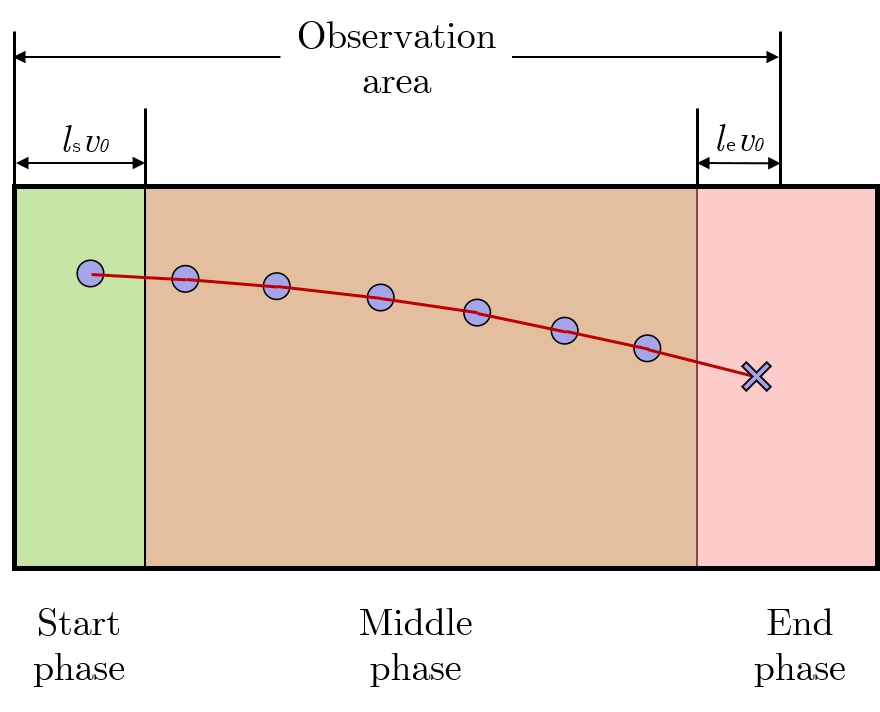
\includegraphics[width=0.4\textwidth]{figures/association area.png}
\caption{The different phase for association. The $l_{\mathrm{s}}$ and $l_{\mathrm{e}}$ determines respectively the range of the start and the end phase.}
\label{asso area}
\end{figure}

However, as shown in Figure \ref{phase}, the default values are different from the ideal values because of the noise, including the difference between the velocity estimation and the real velocity as well as the measurement noise. For example, several measurements belong to the first timestep are misclassified into the middle phase in Figure \ref{phase}a with the ideal boundary. Therefore, we used the $l_{\mathrm{s}}=1.3$ to classify all these measurements into the start phase.

The modified $l_{\mathrm{s}}$ and $l_{\mathrm{e}}$ can also increase the possibility of the misclassification of the measurements and predictions into the wrong phases, which can cause the track separating into two tracks in the start and end area as shown in Figure \ref{association error example}a. But this type of error can be suppressed with a higher $d_{\mathrm{am}}$ and $d_{\mathrm{dm}}$ according to Equation \eqref{assoeq1}. However, shortened start and end phases are hard to compensate with adjusting the other association hyperparameters. Nevertheless, a lower coefficient is still suggested for increasing the robustness of the association. To reduce the influence of the inaccurate initial velocity guess given by the user, the refined initial velocity guess should also be applied to the calculation of the boundary locations. With the refined initial velocity, the possibility for the misdivision of measurements into the middle phase is lowered, and the coefficient can be also lower, just like the refined initial velocity variance in the prediction part.

\begin{figure}[htbp]
	\centering
	\begin{subfigure}[t]{0.45\textwidth}
		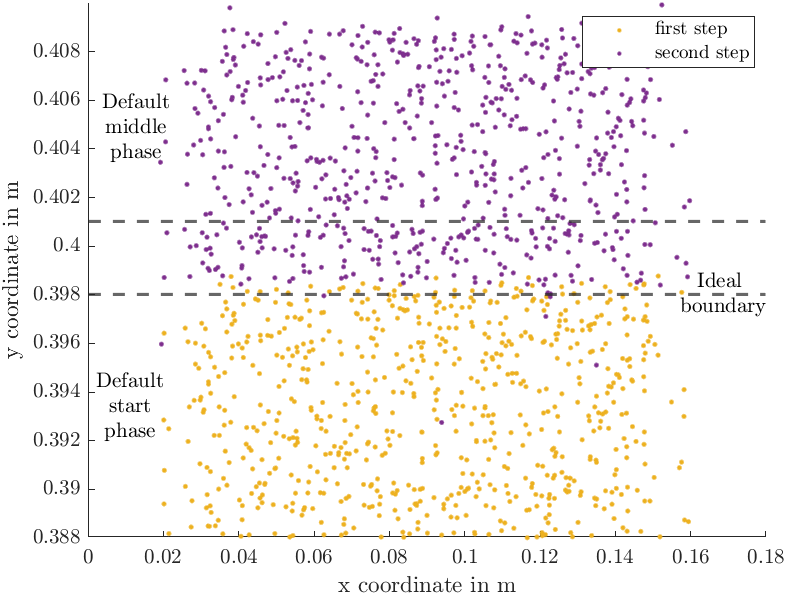
\includegraphics[width=\textwidth]{figures/Asso/range 1.png}
		\caption{The distribution of measurements at the first and second step in the track.}
	\end{subfigure}
	\quad
	\begin{subfigure}[t]{0.45\textwidth}
		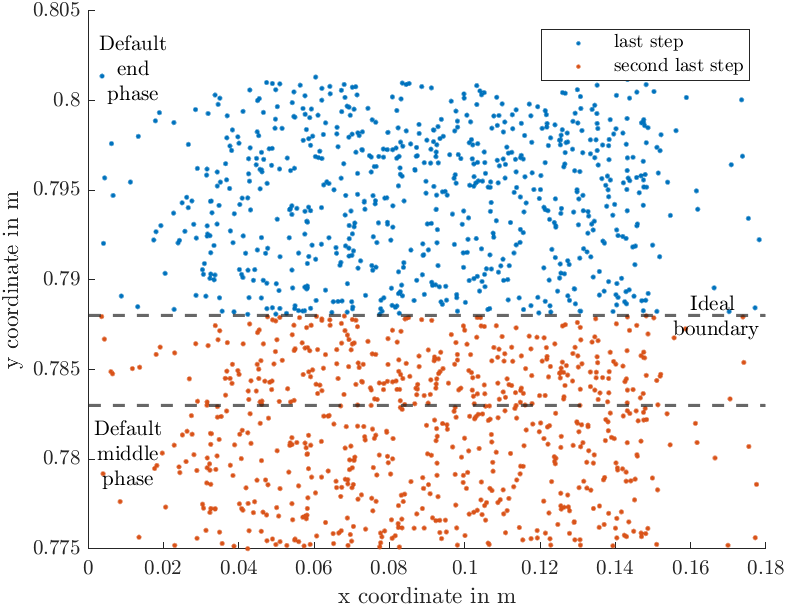
\includegraphics[width=\textwidth]{figures/Asso/range 2.png}
		\caption{The distribution of predictions at the last and second last step in the track.}
	\end{subfigure}
	\caption{Distributions of measurements and predictions around the boundary between phases.}
	\label{phase}
\end{figure}

